\chapter{Conception fonctionnelle et technique}
\vspace{-1.5em}
\chaptertoc
\vspace{-2.5em}
\section{Introduction}
Ce chapitre est dédié à la conception fonctionnelle et technique de la plateforme d'analyse des risques de projet. Il détaille dans un premier temps la phase d'analyse des besoins, fruit d'une démarche itérative menée auprès des parties prenantes, avant de définir de manière exhaustive les exigences fonctionnelles et non fonctionnelles. Cette étape fondamentale permet de poser les jalons de l'architecture logicielle qui sera mise en œuvre pour répondre aux problématiques de suivi soulevées par les équipes de NTT DATA Maroc.

\section{Analyse des besoins}

\subsection{Processus d'identification des besoins}
Le processus de recueil des exigences s'est appuyé sur une démarche hautement collaborative et itérative, essentielle pour s'aligner sur les réalités du terrain. Plusieurs réunions de cadrage et des revues d'avancement hebdomadaires ont été menées en étroite collaboration avec le management et l'équipe d'encadrement, notamment Monsieur Mohammed Amine Elmeknassi et Monsieur Anis Khairi. Ces échanges se sont déroulés selon un format hybride, alliant des ateliers en présentiel dans les locaux de NTT DATA Maroc à Casablanca et des sessions de travail à distance. L'utilisation systématique de présentations lors de ces points d'étape a permis de valider progressivement les hypothèses de conception et de cerner avec précision les attentes des futurs utilisateurs vis-à-vis de l'automatisation par l'intelligence artificielle.

\subsection{Les besoins fonctionnels}
Les fonctionnalités du système ont été définies en fonction des interactions attendues pour chaque acteur clé de la plateforme. En premier lieu, l'agent d'intelligence artificielle agit comme le moteur d'analyse continu du système ; il a pour mission d'interroger l'API Jira de façon autonome, de traiter les descriptions et les commentaires pour y déceler des anomalies, et de générer des recommandations d'actions correctives. En second lieu, l'utilisateur final nécessite un accès interactif à un tableau de bord global. Cet espace doit lui permettre de visualiser les métriques de performance, de consulter les prévisions de la date de fin générées par les simulations de Monte Carlo, et d'exporter ces indicateurs de manière intuitive. En troisième lieu, l'administrateur doit disposer des interfaces nécessaires pour configurer les paramètres globaux de l'application, gérer les comptes utilisateurs et définir finement les niveaux d'autorisation grâce à un système de contrôle d'accès basé sur les rôles. Enfin, l'acteur DevOps requiert des mécanismes automatisés facilitant le déploiement de l'infrastructure conteneurisée, ainsi que des outils permettant de superviser la bonne exécution des tâches d'arrière-plan.

\subsection{Les besoins non fonctionnels}

Afin de garantir une exploitation fiable et fluide en milieu industriel, l'application doit satisfaire des critères non fonctionnels rigoureux. Sur le plan des performances, le système s'engage à fournir des temps d'affichage minimaux de l'interface, rendus possibles par l'implémentation d'un système de mise en cache Redis qui évite le recalcul des métriques lourdes. La sécurité constitue une priorité absolue ; elle est assurée par une authentification stricte basée sur des jetons JWT et par l'utilisation d'un modèle de langage hébergé localement, garantissant ainsi qu'aucune donnée de projet confidentielle ne transite vers des serveurs externes. En matière de disponibilité, la plateforme est conçue pour fonctionner de manière ininterrompue en arrière-plan, s'appuyant sur des processus asynchrones qui assurent un service en continu. La maintenabilité est assurée par une architecture logicielle modulaire séparant clairement l'interface utilisateur des logiques de l'agent IA, facilitant ainsi l'ajout futur de nouveaux indicateurs. L'utilisabilité a été pensée pour offrir une expérience visuelle moderne, favorisant une interprétation instantanée des graphiques complexes. Enfin, l'interopérabilité est garantie par le respect strict des standards d'interface de programmation, permettant au système de s'intégrer de manière transparente avec l'écosystème Jira de l'entreprise.

\section{Analyse de l'existant}

Avant de proposer une solution d’optimisation, il est essentiel d’analyser l’existant afin d’identifier
les forces et les limites du système actuellement en place.

\subsection{Étude de l'existant}
Au sein de NTT DATA Maroc, le pilotage des projets et l'analyse des risques reposent historiquement sur une exploitation classique des outils de gestion de cycle de vie des applications, principalement Jira. Les chefs de projet s'appuient sur les tableaux de bord natifs de la plateforme pour suivre l'avancement global des tâches et identifier visuellement les éventuels points de blocage. Pour répondre aux exigences de reporting du top management, cette approche est couramment complétée par des extractions manuelles de données vers des tableurs Excel, qui sont ensuite souvent intégrées dans des solutions de type Power BI. Ces données agrégées servent finalement de support lors des revues d'avancement hebdomadaires sous forme de présentations. Par ailleurs, bien que des extensions spécialisées du marché telles que BigPicture, EazyBI ou Risk Explorer soient reconnues pour offrir des capacités avancées de visualisation et de gestion de portefeuille, elles demeurent fondamentalement orientées vers l'analyse rétrospective. Actuellement, la détection des risques repose donc presque exclusivement sur l'expertise humaine des chefs de projet, qui doivent examiner individuellement l'état des tickets, vérifier leur ancienneté et interpréter les commentaires pour évaluer la santé réelle d'un projet de développement.

\begin{figure}[!h]
	\centering
	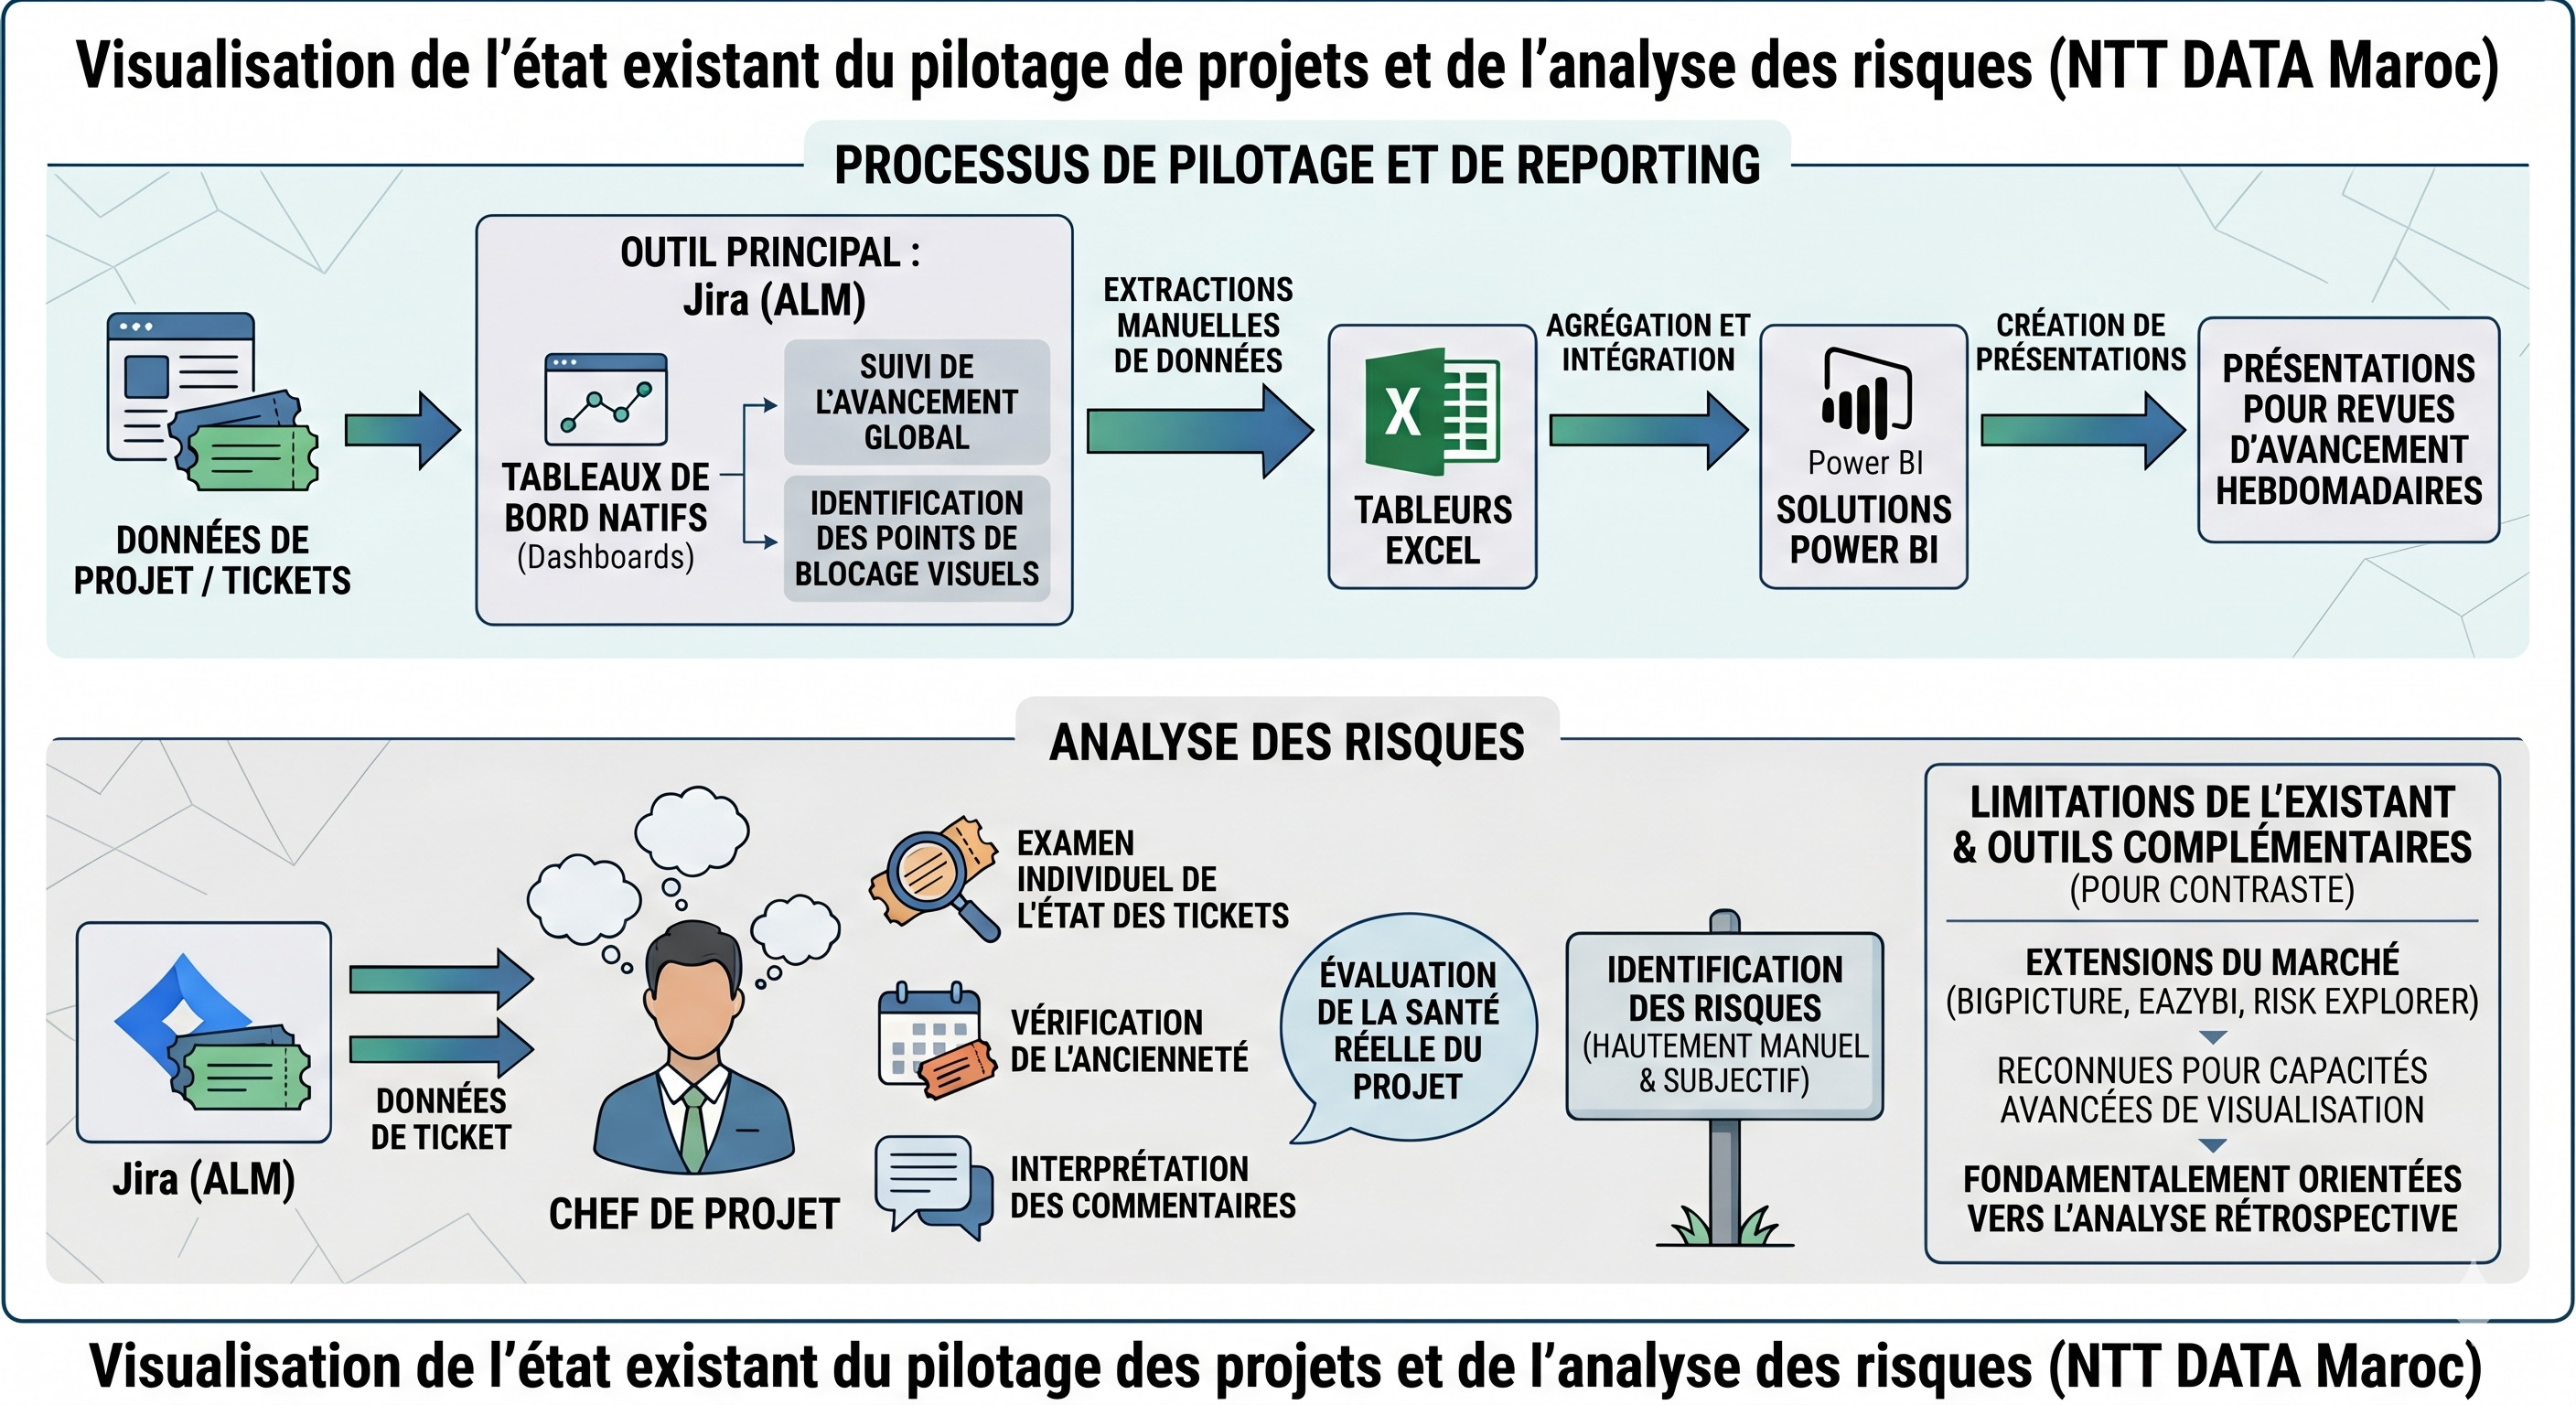
\includegraphics[width=0.9\linewidth]{assets/state_of_existance.png}
	\caption{State of Existance}
	\label{fig:state_existance}
\end{figure}

\subsection{Identification des limitations de l'existant}
Cette approche traditionnelle présente plusieurs limitations majeures qui entravent l'efficacité opérationnelle et la réactivité des équipes :
\begin{enumerate}
    \item \textbf{Caractère hautement chronophage et manuel} : la collecte des indicateurs est une tâche répétitive qui mobilise un temps précieux au détriment de la prise de décision stratégique.
    \item \textbf{Manque d’outils d’analyse prédictive} : l’absence de modèles probabilistes robustes, tels que les simulations de Monte Carlo, oblige les gestionnaires à formuler des estimations de délais basées sur l’intuition plutôt que sur des projections statistiques rigoureuses.
    \item \textbf{Incapacité à exploiter la sémantique des données textuelles} : sans l’apport de l’intelligence artificielle, il est impossible de traiter automatiquement le contenu qualitatif des descriptions et des échanges pour y déceler des signes précoces de dette technique, d’incompréhension des spécifications ou de blocages invisibles.
    \item \textbf{Absence de génération automatique de recommandations} : aucune action correctrice n’est proposée de manière autonome, laissant le chef de projet seul face à l’élaboration de solutions de remédiation.
    \item \textbf{Réaction tardive aux problèmes émergents} : l’absence d’automatisation intelligente fait que les risques ne sont souvent traités qu’après s’être transformés en incidents impactant le calendrier ou le budget.
    \item \textbf{Surcharge cognitive et risque d’omission} : face à l’augmentation constante du volume de tickets dans les projets complexes, l’analyse exclusivement humaine provoque une charge mentale inévitable, augmentant le risque d’oublier des informations critiques.
\end{enumerate}


\subsection{Vue d'ensemble}
Pour répondre aux exigences complexes de l'analyse prédictive et de l'automatisation du suivi de projet, la plateforme s'articule autour d'une architecture distribuée, modulaire et hautement intégrée. Cette conception vise à séparer clairement les responsabilités (extraction de données, calcul intensif, raisonnement par intelligence artificielle et présentation visuelle) afin de garantir à la fois la scalabilité du système, la sécurité absolue des données sensibles et la fluidité de l'interface utilisateur. L'ensemble interagit au travers d'interfaces de programmation (API) standardisées, permettant une évolution indépendante de chaque composant.

\begin{figure}[H]
\centering
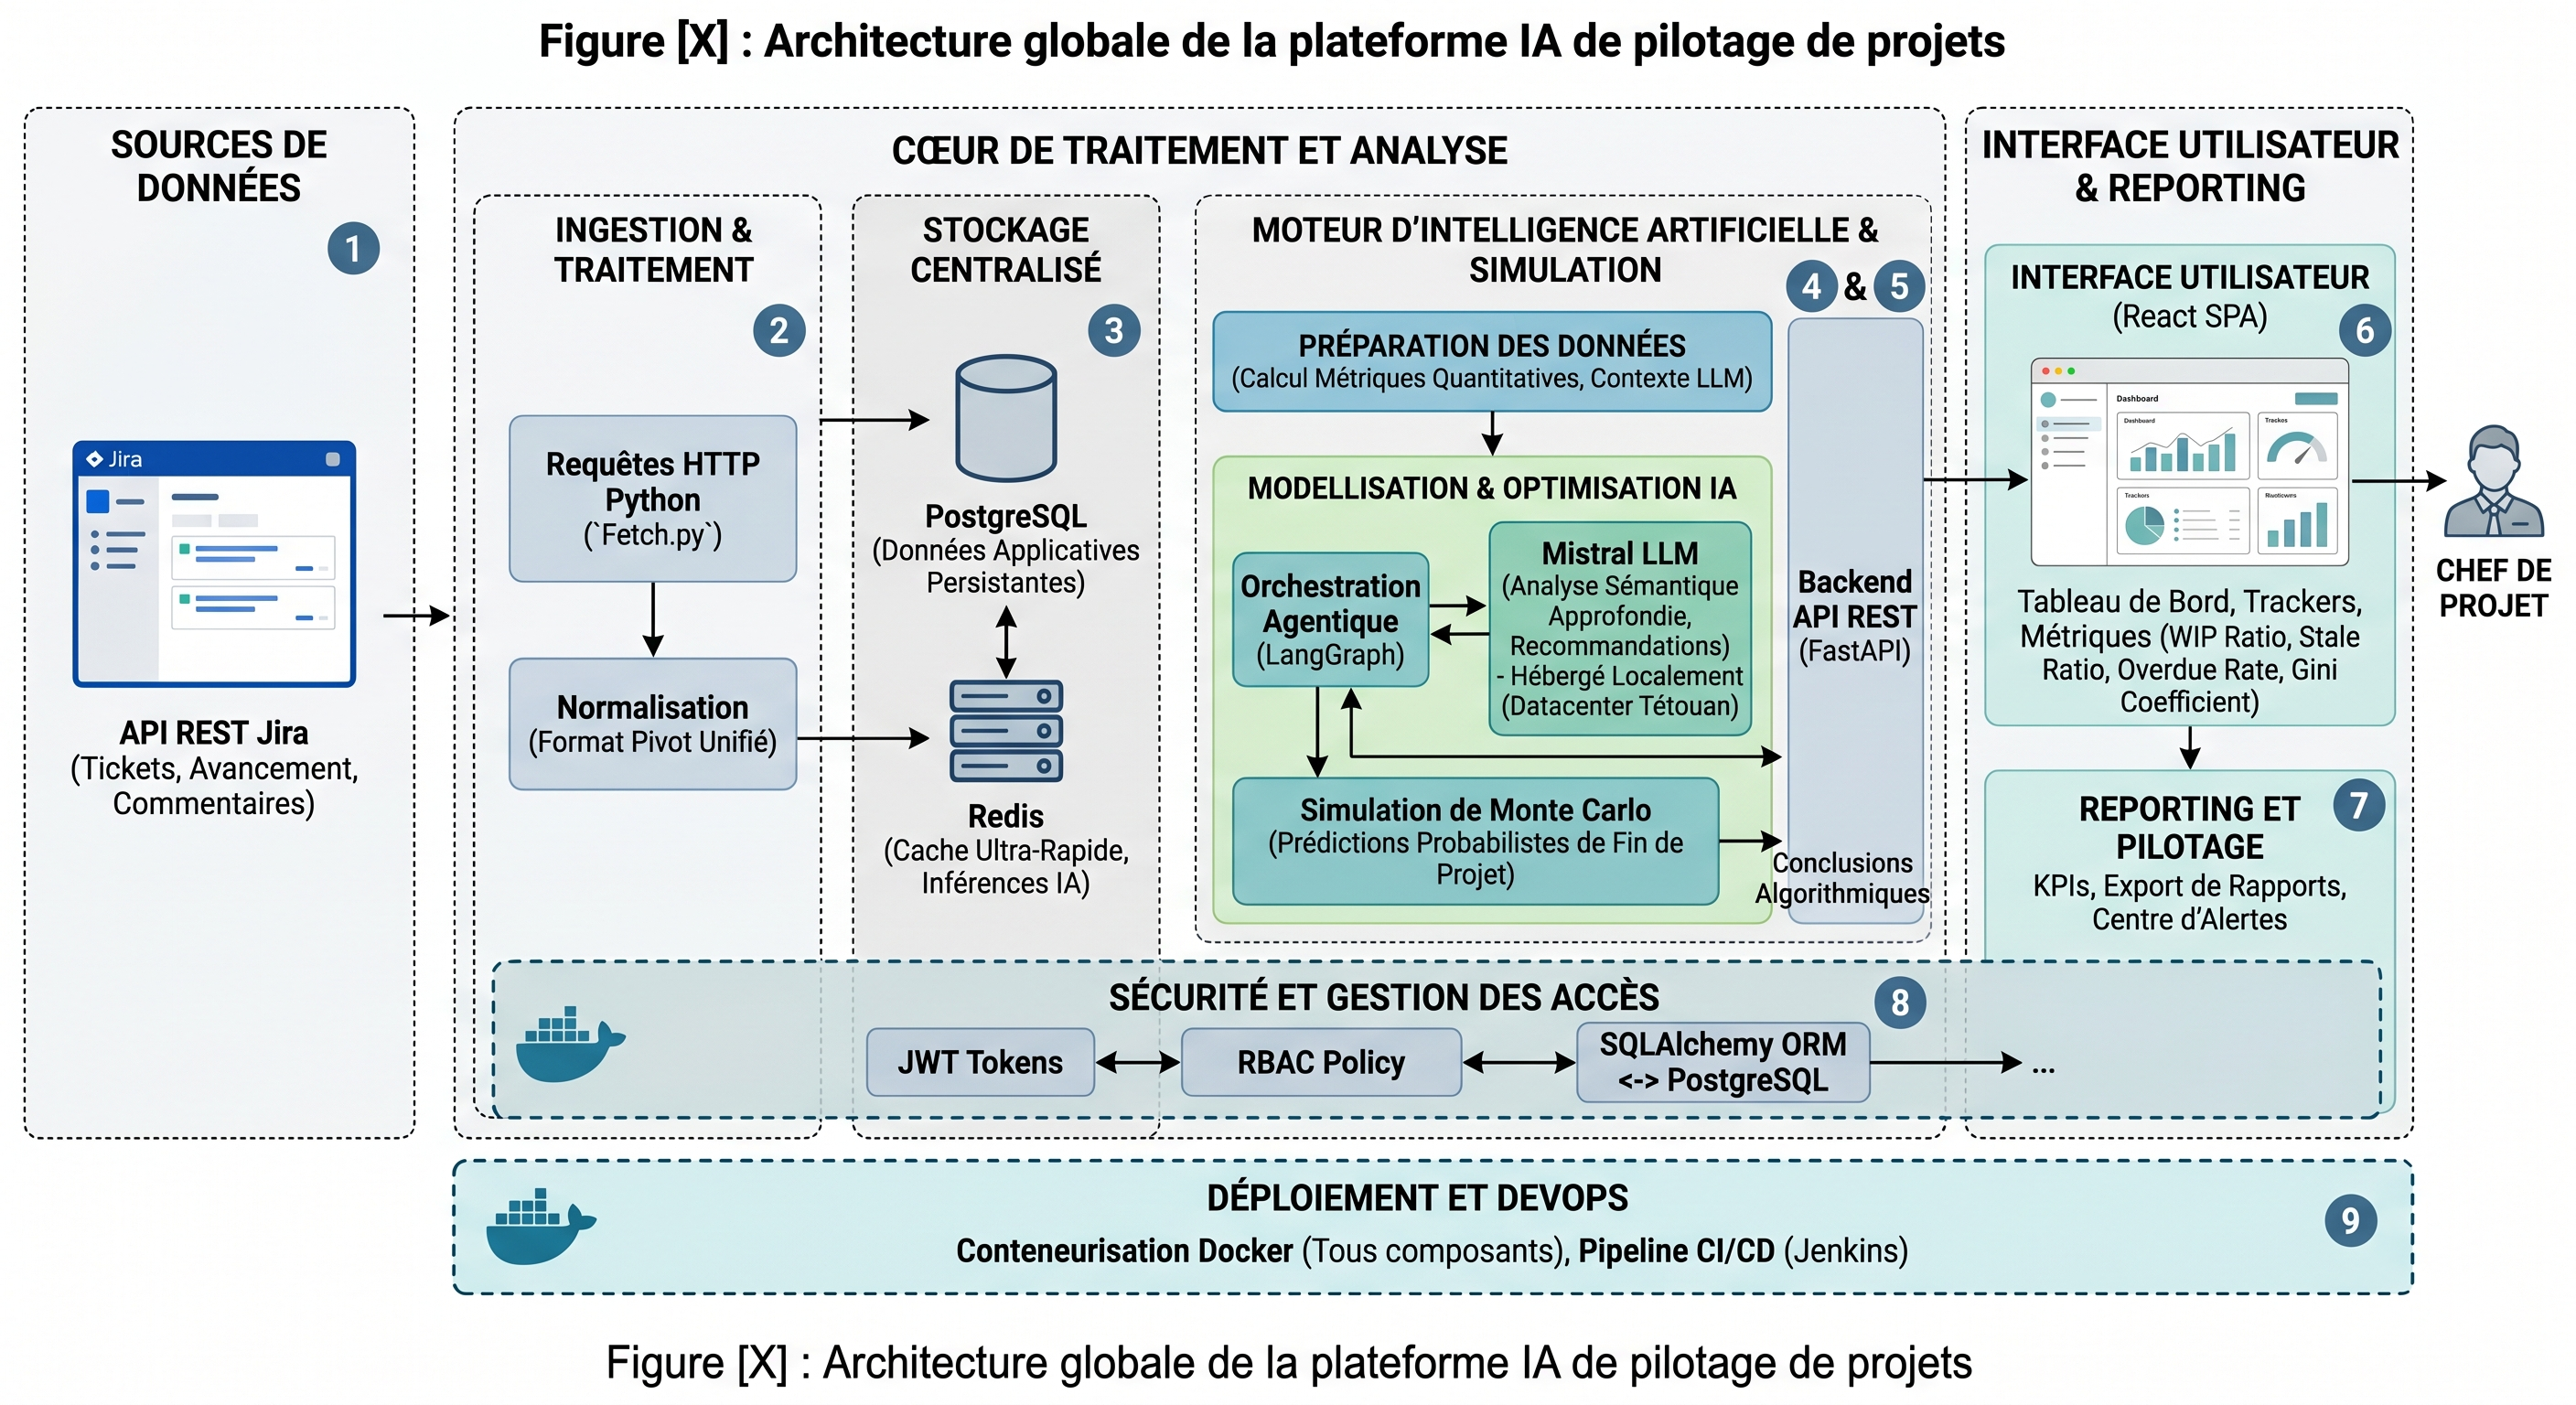
\includegraphics[width=0.9\linewidth]{assets/architecture_globale.png}
\caption{Architecture globale de la plateforme IA de pilotage de projets}
\label{fig:archi_globale}
\end{figure}

L'architecture se compose des éléments suivants :
\begin{enumerate}
\item \textbf{Sources de données :} L'application interagit en premier lieu avec l'API REST de Jira. Cette interface constitue la source de vérité externe, fournissant l'exhaustivité des informations relatives à la gestion de projet (détail des tickets, statuts d'avancement, assignations, historiques de transition et commentaires).
\item \textbf{Ingestion et traitement des données :} La récupération des données brutes est assurée de manière programmatique via des requêtes HTTP en Python. Des modules spécifiques de service (notamment \texttt{Fetch.py}) se chargent ensuite de la normalisation, transformant les structures JSON hétérogènes renvoyées par Jira en un format unifié et exploitable par le cœur de calcul.
\item \textbf{Stockage centralisé :} La persistance des données repose sur une double infrastructure. Une base de données relationnelle PostgreSQL est utilisée pour le stockage persistant et sécurisé des données applicatives (informations utilisateurs, rôles, configurations). En parallèle, un système en mémoire Redis est déployé en tant que cache ultra-rapide pour stocker les calculs statistiques et les inférences de l'IA, évitant ainsi la latence des recalculs.
\item \textbf{Moteur d'intelligence artificielle :} Véritable cerveau du système, ce moteur associe un système de règles déterministes à une approche agentique orchestrée par le framework LangGraph. L'analyse sémantique approfondie est déléguée au modèle de langage large (LLM) Mistral. Pour des raisons strictes de conformité et de protection des données, ce modèle est physiquement hébergé sur les serveurs locaux de NTT DATA au datacenter de Tétouan.
\item \textbf{Moteur de simulation :} Afin d'apporter une dimension prédictive au suivi, un moteur de simulation de Monte Carlo est implémenté en Python, tirant parti de bibliothèques de calcul scientifique telles que NumPy et Pandas. Ce moteur génère des scénarios probabilistes basés sur les durées historiques des tâches pour anticiper de manière réaliste la date d'achèvement d'un projet.
\item \textbf{Interface utilisateur :} L'interaction avec le chef de projet est matérialisée par une application web dynamique (Single Page Application) construite avec la bibliothèque React. Elle héberge le tableau de bord principal et des explorateurs spécifiques, affichant en temps réel des métriques avancées telles que le ratio des travaux en cours (WIP ratio), le taux de tickets obsolètes (stale ratio), le taux de retard (overdue rate) et le coefficient d'inégalité de Gini.
\item \textbf{Reporting et pilotage :} Le tableau de bord agit comme la tour de contrôle du projet en agrégeant les indicateurs de performance clés (KPI) au sein de grilles graphiques et de diagrammes. Il intègre un système de boutons d'exportation pour le reporting de direction, ainsi qu'un centre d'alertes affichant directement les recommandations de l'IA.
\item \textbf{Sécurité et gestion des accès :} La sécurisation des points de terminaison est garantie par un mécanisme de jetons JSON Web Tokens (JWT). Une politique stricte de contrôle d'accès basé sur les rôles (RBAC) est mise en place, avec un mappage des droits géré par l'ORM SQLAlchemy communiquant avec la base PostgreSQL.
\item \textbf{Déploiement et DevOps :} Afin d'assurer une reproductibilité sans faille entre le développement et l'infrastructure client, l'ensemble des composants (frontend, backend FastAPI, bases de données) est encapsulé dans des conteneurs Docker. Le cycle de livraison est orchestré par un pipeline d'intégration et de déploiement continus (CI/CD) opéré sous Jenkins.
\end{enumerate}

\subsection{Zoom sur l'architecture du module d'intelligence artificielle}
Le module d'intelligence artificielle constitue le noyau prédictif et qualitatif de la plateforme. Conçu pour dépasser la simple agrégation statistique, il agit comme un véritable agent expert autonome, capable de déduire des risques systémiques en croisant des données mathématiques avec des nuances sémantiques. L'intégration de LangGraph permet spécifiquement de maintenir l'état conversationnel de l'agent, lui conférant une « mémoire » de sa chaîne de raisonnement à travers les différentes étapes de l'analyse.
\begin{figure}[H]
\centering
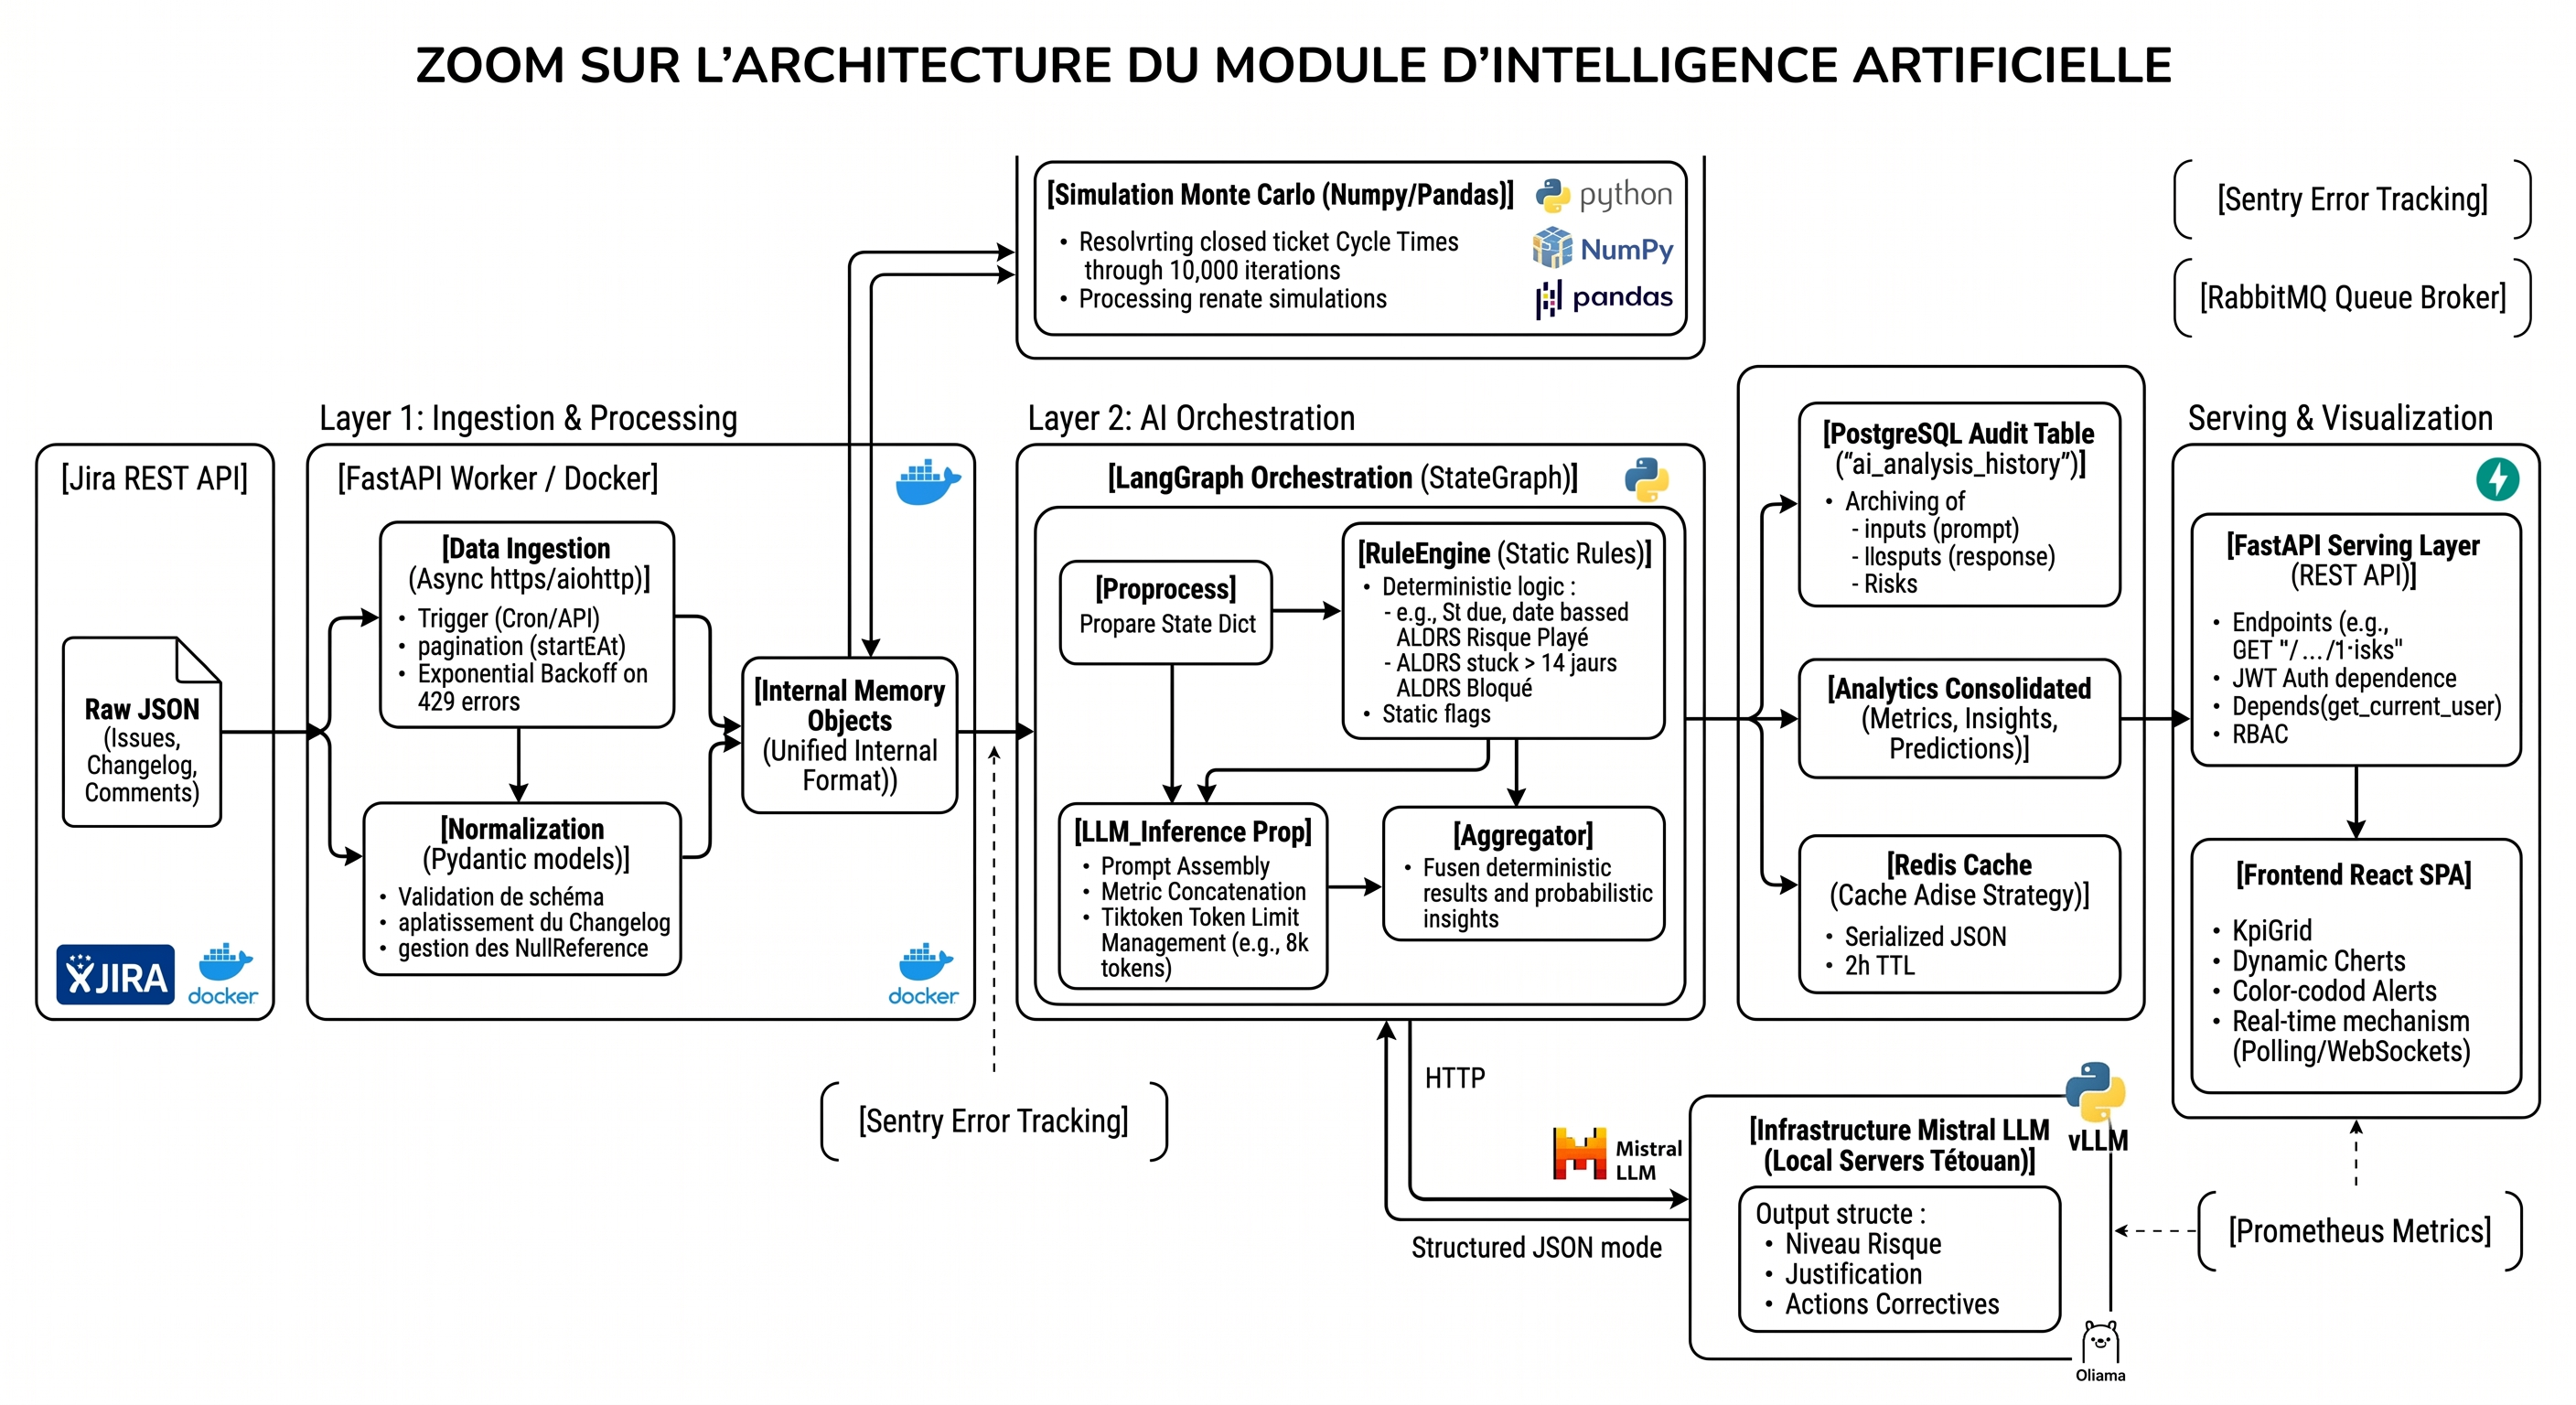
\includegraphics[width=0.9\linewidth]{assets/architecture_ai.png}
\caption{Architecture globale de IA}
\label{fig:archi_ai}
\end{figure}


L'architecture de ce module suit un pipeline structuré en plusieurs phases :
\begin{enumerate}
\item \textbf{Prétraitement et préparation des données}
\begin{itemize}
\renewcommand{\labelitemi}{—}
    \item Extraction asynchrone des données de gestion de projet via l'API REST Jira.
    \item Normalisation des champs pour consolider les structures disparates en un format pivot unifié.
    \item Calcul intensif des métriques quantitatives fondamentales (WIP ratio, stale ratio, overdue rate, coefficient de Gini).
    \item Préparation contextuelle des entrées pour le modèle LLM, impliquant l'assemblage cohérent des descriptions de tâches, des commentaires techniques et des historiques d'évolution.
\end{itemize}

\item \textbf{Modélisation et optimisation IA}
\begin{itemize}
\renewcommand{\labelitemi}{—}
    \item Filtrage préalable par un moteur de règles statiques visant à identifier instantanément les risques évidents (délais structurellement dépassés, tickets bloqués).
    \item Orchestration du flux cognitif par LangGraph, qui encadre la logique de décision et gère l'état d'exécution de l'agent.
    \item Soumission des requêtes au LLM Mistral (hébergé en circuit fermé à Tétouan) pour effectuer une analyse sémantique des échanges et générer des recommandations d'actions correctives.
    \item Exécution de la simulation de Monte Carlo pour déduire, à partir de la variance historique, une prédiction probabiliste de la date de fin de projet.
\end{itemize}

\item \textbf{Déploiement via API et conteneurisation}
\begin{itemize}
\renewcommand{\labelitemi}{—}
    \item Exposition unifiée des conclusions algorithmiques (scores de risques, textes de recommandation, intervalles de confiance prédictifs) par l'intermédiaire d'une API REST développée avec le framework asynchrone FastAPI.
    \item Isolation du processus analytique au sein d'un environnement conteneurisé Docker.
\end{itemize}

\item \textbf{Intégration applicative et visualisation}
\begin{itemize}
\renewcommand{\labelitemi}{—}
    \item Transmission asynchrone des résultats d'analyse vers le système de cache Redis, garantissant une mise à disposition véloce au backend.
    \item Restitution visuelle et interprétation dans le tableau de bord React, traduisant les vecteurs de données en éléments d'interface lisibles (alertes, recommandations, graphiques dynamiques).
    \item Maintien d'une traçabilité des décisions algorithmiques et conservation de l'historique des analyses.
\end{itemize}
\end{enumerate}


\section{Environnements logiciels et technologies}
Cette section présente les outils, langages et environnements utilisés au cours du projet, en justifiant les choix technologiques réalisés à chaque étape. Une veille technologique a également été menée dans le cadre de l’exploration des solutions open-source pour l’orchestration d’agents IA et l’hébergement local de modèles de langage.

\subsection{Technologies utilisées}
Afin de mettre en œuvre le projet selon l’architecture définie, nous avons mobilisé plusieurs technologies :

\textbf{Python} — Langage principal utilisé pour le développement du backend et du module d’intelligence artificielle. Python a été choisi pour sa flexibilité, sa lisibilité, ainsi que la richesse de son écosystème scientifique. Les bibliothèques suivantes ont été mobilisées :

\begin{figure}[H]
\centering

\includegraphics[width=0.2\linewidth]{assets/logos/python.png}
\caption{Python}
\label{fig:Python}
\end{figure}

\begin{itemize}
\renewcommand{\labelitemi}{—}
    \item \textbf{FastAPI} : framework asynchrone pour la création d’API RESTful, facilitant l’exposition des services IA et l’intégration avec le frontend React.
    \begin{figure}[H]
    \centering
    
\includegraphics[width=0.2\linewidth]{assets/logos/fastApi.png}
    \caption{Python fast api}
    \label{fig:Python_fastapi}
    \end{figure}
    \item \textbf{SQLAlchemy} : ORM utilisé pour interagir avec la base de données PostgreSQL, permettant une gestion élégante des modèles utilisateurs et des rôles RBAC.
    \begin{figure}[H]
    \centering
    
\includegraphics[width=0.2\linewidth]{assets/logos/sqlalchemy.jpg}
    \caption{sqlalchemy}
    \label{fig:sqlalchemy}
    \end{figure}
    \item \textbf{LangGraph} : framework d’orchestration d’agents IA, retenu pour sa capacité à maintenir un état conversationnel et à gérer des flux de décision cycliques.
    \begin{figure}[H]
    \centering
    
\includegraphics[width=0.2\linewidth]{assets/logos/langgraph.png}
    \caption{Python langgraph}
    \label{fig:Python_langgraph}
    \end{figure}
    \item \textbf{Mistral} : modèle de langage large (LLM) hébergé localement sur les serveurs de Tétouan, choisi pour son équilibre entre performance et confidentialité des données.
    \begin{figure}[H]
    \centering
    
\includegraphics[width=0.2\linewidth]{assets/logos/mistral.jpeg}
    \caption{Python}
    \label{fig:Python_mistral}
    \end{figure}
    \item \textbf{NumPy, Pandas} : bibliothèques de calcul scientifique utilisées pour les simulations de Monte Carlo et le calcul des métriques (WIP ratio, stale ratio, coefficient de Gini).
    \begin{figure}[H]
    \centering
    
\includegraphics[width=0.2\linewidth]{assets/logos/numpy.jpg}
    \caption{Python numpy}
    \label{fig:Python_numpy}
    \end{figure}
\end{itemize}

\textbf{React} — Bibliothèque JavaScript utilisée pour le développement du tableau de bord interactif. React permet une expérience utilisateur réactive et une visualisation en temps réel des métriques et alertes.

\begin{figure}[H]
\centering

\includegraphics[width=0.2\linewidth]{assets/logos/react_logo.png}
\caption{react}
\label{fig:react}
\end{figure}

\textbf{PostgreSQL} — Système de gestion de base de données relationnelle, retenu pour sa robustesse et sa conformité aux exigences de sécurité (stockage des identifiants, rôles et configurations).

\begin{figure}[H]
\centering

\includegraphics[width=0.3\linewidth]{assets/logos/postgres_logo.png}
\caption{postgres}
\label{fig:postgres}
\end{figure}

\textbf{Redis} — Système de cache en mémoire déployé pour accélérer l’accès aux résultats des analyses IA et aux métriques fréquemment sollicitées, réduisant ainsi la latence du tableau de bord.

\begin{figure}[H]
\centering

\includegraphics[width=0.2\linewidth]{assets/logos/redis.png}
\caption{redis}
\label{fig:redis}
\end{figure}

\textbf{Docker} — Outil de conteneurisation permettant d’encapsuler l’ensemble des composants (backend FastAPI, frontend React, base de données) dans des environnements isolés et reproductibles.

\begin{figure}[H]
\centering

\includegraphics[width=0.2\linewidth]{assets/logos/docker.png}
\caption{docker}
\label{fig:docker}
\end{figure}

\textbf{Jenkins} — Serveur d’intégration continue utilisé pour automatiser les pipelines CI/CD, assurant les tests, la construction et le déploiement de la plateforme.
\begin{figure}[H]
\centering

\includegraphics[width=0.4\linewidth]{assets/logos/jenkins.jpg}
\caption{jenkins}
\label{fig:jenkins}
\end{figure}

\subsection{Technologies utilisées par l’équipe de développement}
L’équipe de développement a utilisé un ensemble d’outils collaboratifs et d’environnements de travail :
\begin{itemize}
\renewcommand{\labelitemi}{—}
    \item \textbf{Visual Studio Code} : IDE principal, apprécié pour ses extensions Python, son débogueur intégré et son terminal facilitant les tests.
    \begin{figure}[H]
    \centering
    
\includegraphics[width=0.2\linewidth]{assets/logos/vsCode.png}
    \caption{vs}
    \label{vs}
    \end{figure}
    \item \textbf{GitLab} : plateforme de gestion de version basée sur Git, utilisée pour le suivi des modifications du code source et la collaboration entre développeurs, accessible à l’adresse \href{https://umane.emeal.nttdata.com/git/FELTRIINTPROJ/nttdata-ai-agent-project-tracking}{https://umane.emeal.nttdata.com/git/FELTRIINTPROJ/nttdata-ai-agent-project-tracking}.    \item \textbf{Microsoft Teams} : outil de communication quotidienne pour les réunions de synchronisation (daily stand-ups) et les échanges avec l’encadrement.
    \begin{figure}[H]
    \centering
    
\includegraphics[width=0.2\linewidth]{assets/logos/gitlab_logo.png}
    \caption{gitlab}
    \label{fig:gitlab}
    \end{figure}
    \item \textbf{Jira} : utilisé pour le suivi des tâches du projet lui-même, accessible à l’adresse \href{https://umane.emeal.nttdata.com/jiraito/browse/HPCMOROCCO}{https://umane.emeal.nttdata.com/jiraito/browse/HPCMOROCCO}, démontrant ainsi l’adéquation de la plateforme avec les méthodes agiles.    \item \textbf{Postman} : outil de test d’API REST, employé pour valider les endpoints FastAPI avant intégration.
    \begin{figure}[H]
    \centering
    
\includegraphics[width=0.2\linewidth]{assets/logos/jira_logo.png}
    \caption{jira}
    \label{fig:jira}
    \end{figure}
    \item \textbf{Docker Compose} : utilisé en développement pour orchestrer l’exécution simultanée des conteneurs backend, frontend, PostgreSQL et Redis.
    \begin{figure}[H]
    \centering
    
\includegraphics[width=0.2\linewidth]{assets/logos/docker.png}
    \caption{docker}
    \label{fig:docker}
    \end{figure}
\end{itemize}

\subsection{Veille technologique sur les agents IA conversationnels pour l’analyse de projets}
Dans le cadre de l’exploration des solutions open-source pour l’analyse automatisée des risques à partir de données Jira, une veille technologique a été menée. Plusieurs technologies ont été examinées :
\begin{itemize}
\renewcommand{\labelitemi}{—}
    \item \textbf{LangChain} : framework populaire pour la construction d’applications LLM, mais moins adapté aux graphes d’état complexes.
    \begin{figure}[H]
    \centering
    
\includegraphics[width=0.2\linewidth]{assets/logos/langchain.png}
    \caption{langchain}
    \label{fig:langchain}
    \end{figure}
    \item \textbf{LlamaIndex} : spécialisé dans l’indexation et la récupération de documents, sans capacité native d’orchestration d’agents.
    \begin{figure}[H]
    \centering
    
\includegraphics[width=0.2\linewidth]{assets/logos/llamaindex_logo.png}
    \caption{llama}
    \label{fig:llama}
    \end{figure}
    \item \textbf{Rasa} : conçu pour les chatbots conversationnels, mais trop lourd et non orienté vers l’analyse de données structurées de gestion de projet.
    \begin{figure}[H]
    \centering
    
\includegraphics[width=0.2\linewidth]{assets/logos/rasa_logo.png}
    \caption{rasa}
    \label{fig:rasa}
    \end{figure}
    \item \textbf{Mistral vs. LLaMA 3} : comparaison de modèles de langage open-source pouvant être hébergés localement.
    \begin{figure}[H]
    \centering
    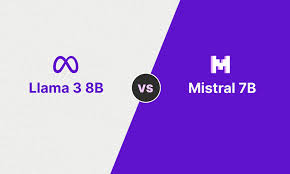
\includegraphics[width=0.2\linewidth]{assets/logos/llama_mistral.jpg}
    \caption{llama_index}
    \label{fig:llama_index}
    \end{figure}
\end{itemize}
À l’issue de cette veille, \textbf{LangGraph} a été retenu pour l’orchestration de l’agent IA, et \textbf{Mistral} pour le LLM, en raison de sa faible empreinte mémoire et de son excellente gestion de la langue française.

\subsection{Comparaison des outils d’orchestration d’agents IA}
Le tableau \ref{tab:comparaison_orchestration} présente une comparaison synthétique entre deux frameworks d’orchestration envisagés : LangChain et LangGraph.

\begin{table}[H]
\centering
\renewcommand{\arraystretch}{1.2}
\caption{Comparaison entre LangChain et LangGraph}
\begin{tabular}{|l|l|l|}
\hline
\textbf{Critère} & \textbf{LangChain} & \textbf{LangGraph} \\
\hline
Nature & Chaînes linéaires & Graphes d’état cycliques \\
Gestion de la mémoire & Limitée (contextuelle) & Native (état persistant) \\
Adaptation aux agents autonomes & Modérée & Excellente \\
Cycles et boucles de décision & Non supporté & Supporté nativement \\
Courbe d’apprentissage & Faible à modérée & Modérée \\
Intégration avec FastAPI & Bonne & Très bonne \\
\hline
\end{tabular}
\label{tab:comparaison_orchestration}
\end{table}

La comparaison montre que LangGraph, bien qu’étant plus récent, est mieux adapté à notre besoin d’un agent conversationnel autonome capable de maintenir un état de raisonnement sur plusieurs cycles d’analyse. LangGraph a donc été retenu pour le développement du module IA.

\subsection{Conclusion}
Ce chapitre a présenté la conception fonctionnelle et technique de notre solution, en partant de l’analyse des besoins jusqu’au choix des technologies. Nous avons détaillé l’architecture globale du système ainsi que celle du module d’intelligence artificielle. Une étude comparative des outils d’orchestration d’agents IA a également permis de justifier les choix technologiques retenus.

Le chapitre suivant portera sur l’implémentation détaillée de la plateforme, décrivant les algorithmes mis en œuvre, l’intégration des composants, ainsi que les résultats obtenus lors des phases de test et de validation.